% !TeX root=../main.tex
\chapter{راهنمای فنی}\label{Chap:TechnicalGuide}

این فصل روش آماده‌سازی محیط توسعه و اجرای محلی سامانهٔ «نوواژه» را توضیح می‌دهد. سامانه از برنامه‌های اندروید و آی‌اواس، کد مشترک و یک کارساز محلی تشکیل شده است. هدف این راهنما آن است که توسعه‌دهنده بتواند با کمترین تنظیم اضافی، وابستگی‌ها را دریافت و همهٔ اجزای اصلی پروژه را اجرا کند.

\section{معماری پروژه}

نوواژه با زبان کاتلین (\lr{Kotlin}) و فناوری کاتلین چندسکویی (\lr{Kotlin Multiplatform} یا \lr{KMP}) توسعه یافته است. رابط کاربری مشترک با کامپوز چندسکویی (\lr{Compose Multiplatform}) ساخته می‌شود و کارساز از چارچوب کِی‌تور (\lr{Ktor}) استفاده می‌کند. فناوری \lr{KMP} امکان اشتراک مدل‌ها، منطق برنامه و بخش زیادی از رابط کاربری میان اندروید (\lr{Android}) و آی‌اواس (\lr{iOS}) را فراهم می‌کند \cite{KotlinMultiplatformDocs2026,KotlinKMPSetup2026}.

شکل \ref{Fig:NovazhehArchitecture} ارتباط میان برنامه‌های موبایل، لایهٔ مشترک، کارساز و منابع دادهٔ محلی را نشان می‌دهد.

\begin{figure}[H]
\centering
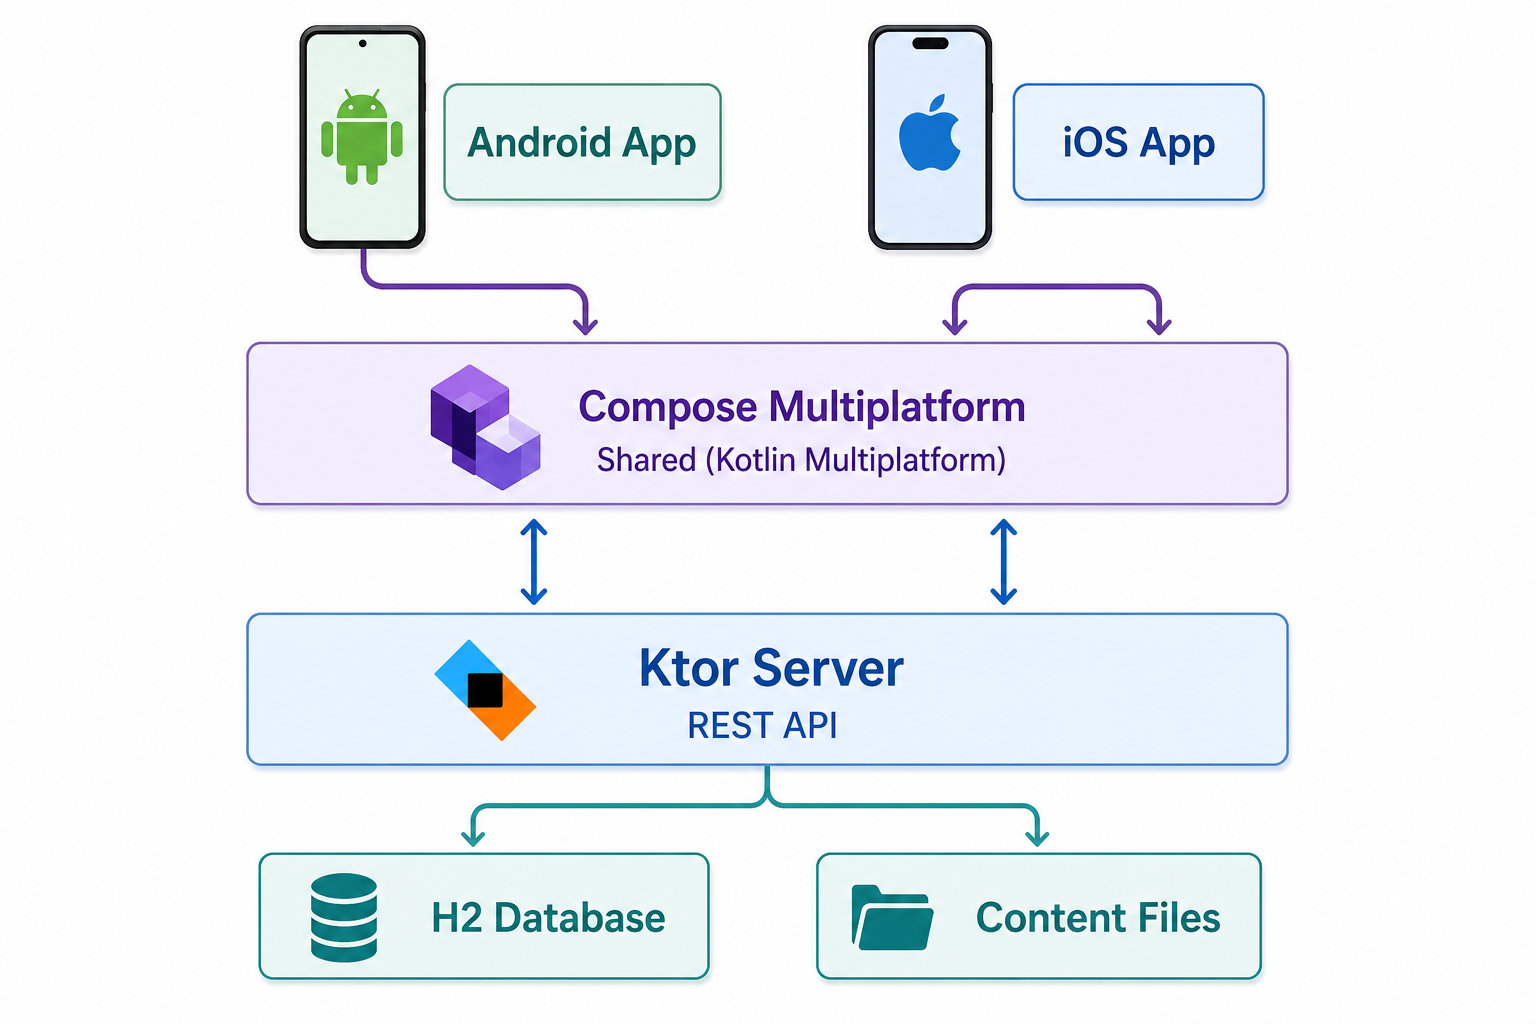
\includegraphics[width=0.95\textwidth]{figures/novazheh-architecture.png}
\caption{معماری کلی سامانهٔ نوواژه}
\label{Fig:NovazhehArchitecture}
\end{figure}

پوشه‌های اصلی پروژه عبارت‌اند از:

\begin{table}[ht]
\centering
\caption{اجزای اصلی پروژهٔ نوواژه}
\label{Tab:RepositoryModules}
\begin{tabular}{|p{0.24\textwidth}|p{0.61\textwidth}|}
\hline
\textbf{مسیر} & \textbf{کاربرد} \\
\hline
\lr{composeApp} & رابط کاربری مشترک و کدهای ویژهٔ اندروید و آی‌اواس \\
\hline
\lr{shared} & مدل‌های داده، ارتباط با کارساز و منطق مشترک برنامه \\
\hline
\lr{server} & کارساز \lr{Ktor}، رابط برنامه‌نویسی (\lr{API})، احراز هویت و داده‌ها \\
\hline
\lr{iosApp} & پروژهٔ میزبان اکس‌کد (\lr{Xcode}) برای ساخت برنامهٔ آی‌اواس \\
\hline
\lr{gradle} & نسخهٔ ابزارها و وابستگی‌های پروژه \\
\hline
\end{tabular}
\end{table}

\section{نسخه‌ها و پیش‌نیازها}

نسخه‌های اصلی ثبت‌شده در پروژه در جدول \ref{Tab:TechnicalVersions} آمده‌اند. هماهنگی این نسخه‌ها برای جلوگیری از خطاهای ساخت ضروری است.

\begin{table}[ht]
\centering
\caption{نسخه‌های اصلی پروژه}
\label{Tab:TechnicalVersions}
\begin{tabular}{|p{0.43\textwidth}|p{0.28\textwidth}|}
\hline
\textbf{ابزار} & \textbf{نسخه} \\
\hline
کاتلین (\lr{Kotlin}) & \lr{2.2.21} \\
\hline
کامپوز چندسکویی (\lr{Compose Multiplatform}) & \lr{1.9.3} \\
\hline
کی‌تور (\lr{Ktor}) & \lr{3.3.3} \\
\hline
افزونهٔ اندروید گرادل (\lr{Android Gradle Plugin}) & \lr{8.11.2} \\
\hline
گرادل (\lr{Gradle Wrapper}) & \lr{8.14.3} \\
\hline
نسخهٔ ساخت و هدف اندروید & \lr{API 36} \\
\hline
کمینهٔ نسخهٔ اندروید & \lr{API 24} \\
\hline
کمینهٔ نسخهٔ استقرار آی‌اواس & \lr{18.2} \\
\hline
\end{tabular}
\end{table}

برای توسعهٔ اندروید و کارساز می‌توان از ویندوز (\lr{Windows})، لینوکس (\lr{Linux}) یا مک‌اواس (\lr{macOS}) استفاده کرد. ساخت آی‌اواس تنها روی مک‌اواس و با اکس‌کد امکان‌پذیر است. ابزارهای لازم عبارت‌اند از:

\begin{itemize}
\item اندروید استودیو (\lr{Android Studio})؛
\item کیت توسعهٔ جاوا ۱۷ (\lr{JDK 17}) برای اجرای گرادل؛
\item کیت توسعهٔ اندروید (\lr{Android SDK 36}) و ابزارهای ساخت؛
\item شبیه‌ساز اندروید (\lr{Android Emulator})؛
\item افزونهٔ کاتلین چندسکویی (\lr{Kotlin Multiplatform Plugin})؛
\item برای آی‌اواس: مک‌اواس، اکس‌کد و شبیه‌ساز آی‌اواس (\lr{iOS Simulator})؛
\item اتصال اینترنت پایدار برای دریافت گرادل و وابستگی‌ها.
\end{itemize}

گرچه کد اندروید برای سطح زبان جاوا ۱۱ ساخته می‌شود، خود افزونهٔ اندروید باید با \lr{JDK 17} اجرا شود \cite{AndroidAGPJDK2026}. بهتر است از جاوای همراه اندروید استودیو استفاده شود. نصب اندروید استودیو و اجزای \lr{SDK} باید از توزیع رسمی انجام شود \cite{AndroidStudioInstall2026}.

\section{دریافت وابستگی‌ها در ایران}

وابستگی‌های پروژه از مخزن مرکزی میون (\lr{Maven Central})، مخزن گوگل (\lr{Google Maven}) و درگاه افزونه‌های گرادل (\lr{Gradle Plugin Portal}) دریافت می‌شوند. در ایران ممکن است دسترسی به برخی از این خدمات محدود باشد. در این حالت می‌توان، مطابق قوانین محل استفاده، از شبکهٔ خصوصی مجازی (\lr{VPN}) معتبر یا خدمت رفع تحریم مبتنی بر سامانهٔ نام دامنه (\lr{DNS}) مانند «شکن» استفاده کرد.

وضعیت شکن متغیر است و در زمان نگارش این گزارش، وبگاه رسمی آن از فعال‌نبودن خدمت عمومی به‌علت محدودیت‌های تحمیل‌شده خبر می‌دهد؛ بنابراین باید وضعیت روز در وبگاه رسمی بررسی و در صورت نیاز از راهکار مجاز دیگری استفاده شود \cite{ShecanStatus2026}. راهکار شبکه باید هم برای اندروید استودیو و هم برای خط فرمان فعال باشد.

پس از برقراری اتصال، همگام‌سازی گرادل (\lr{Gradle Sync}) انجام می‌شود. در صورت ناقص‌بودن دریافت‌ها، دستور زیر اجرا می‌شود:

\begin{latin}
\begin{verbatim}
./gradlew --refresh-dependencies
\end{verbatim}
\end{latin}

در ویندوز، فرمان \lr{gradlew.bat} جایگزین \lr{./gradlew} می‌شود. نباید برای رفع محدودیت، مخزن‌های امن \lr{HTTPS} به \lr{HTTP} تبدیل یا کتابخانه‌ها از وبگاه‌های ناشناس دریافت شوند.

\section{تنظیم اندروید استودیو و پروژه}

پوشهٔ اصلی پروژه در اندروید استودیو باز می‌شود. سپس در بخش تنظیمات گرادل، محیط جاوای گرادل (\lr{Gradle JDK}) روی نسخهٔ ۱۷ یا جاوای همراه محیط توسعه قرار می‌گیرد. در مدیر کیت توسعه (\lr{SDK Manager}) نیز موارد زیر نصب می‌شوند:

\begin{itemize}
\item \lr{Android SDK Platform 36}؛
\item ابزارهای سکوی اندروید (\lr{Android SDK Platform-Tools})؛
\item ابزارهای ساخت اندروید (\lr{Android SDK Build-Tools})؛
\item شبیه‌ساز اندروید و یک تصویر سامانهٔ سطح ۳۶.
\end{itemize}

اندروید استودیو معمولاً پروندهٔ \lr{local.properties} را خودکار می‌سازد. اگر این پرونده ایجاد نشد، مسیر محلی \lr{SDK} در آن ثبت می‌شود؛ برای نمونه:

\begin{latin}
\begin{verbatim}
sdk.dir=/Users/developer/Library/Android/sdk
\end{verbatim}
\end{latin}

این مسیر برای هر رایانه متفاوت است. برای ساخت پروژه باید از گرادل رَپِر (\lr{Gradle Wrapper}) موجود در پروژه استفاده شود و نیازی به نصب جداگانهٔ گرادل نیست. برای بررسی محیط می‌توان فرمان زیر را اجرا کرد:

\begin{latin}
\begin{verbatim}
./gradlew --version
\end{verbatim}
\end{latin}

خروجی باید استفاده از جاوا ۱۷ را نشان دهد.

\section{راه‌اندازی محلی کارساز}

برای اجرای محلی، نصب پایگاه دادهٔ جداگانه لازم نیست. کارساز به‌طور پیش‌فرض از پایگاه دادهٔ سبک اچ‌دو (\lr{H2 Database}) استفاده می‌کند و داده‌های لازم را در پروندهٔ محلی نگه می‌دارد. از ریشهٔ پروژه فرمان زیر اجرا می‌شود:

\begin{latin}
\begin{verbatim}
./gradlew :server:run
\end{verbatim}
\end{latin}

کارساز روی درگاه \lr{8080} اجرا می‌شود. پس از شروع، دو نشانی زیر باید در مرورگر بررسی شوند:

\begin{latin}
\begin{verbatim}
http://localhost:8080/health
http://localhost:8080/swagger
\end{verbatim}
\end{latin}

نشانی نخست سلامت کارساز را نشان می‌دهد و نشانی دوم رابط مستندات سوَگِر (\lr{Swagger}) را برای مشاهده و آزمایش مسیرهای \lr{API} باز می‌کند. کارساز، تبدیل داده‌های جِیسون (\lr{JSON}) و مسیرهای وب با \lr{Ktor} پیاده‌سازی شده‌اند \cite{KtorDocs2026,KtorServerSetup2026}.

پوشهٔ \lr{server/content} شامل محتوای رسانه‌ای برنامه است. نشانی پایهٔ محتوا با متغیر محیطی زیر تعیین می‌شود. مقدار پیش‌فرض برای شبیه‌ساز اندروید مناسب است:

\begin{latin}
\begin{verbatim}
CONTENT_BASE_URL=http://10.0.2.2:8080
\end{verbatim}
\end{latin}

تنظیم پایگاه دادهٔ پستگرس‌کیوال (\lr{PostgreSQL}) اختیاری است و برای راه‌اندازی محلی توصیه نمی‌شود. در صورت استفاده از پایگاه دادهٔ خارجی، گزینهٔ \lr{USE\_POSTGRES} و اطلاعات اتصال آن تنظیم می‌شوند. در محیط واقعی نیز کلید پیش‌فرض احراز هویت باید با یک مقدار قوی و محرمانه جایگزین شود.

\section{اجرای برنامهٔ اندروید}

پس از اجرای کارساز، در مدیر دستگاه (\lr{Device Manager}) یک دستگاه مجازی اندروید (\lr{Android Virtual Device} یا \lr{AVD}) با سطح ۳۶ ساخته می‌شود. سپس پیکربندی \lr{composeApp} و شبیه‌ساز انتخاب و برنامه اجرا می‌گردد. برای ساخت نسخهٔ اشکال‌زدایی از خط فرمان نیز می‌توان نوشت:

\begin{latin}
\begin{verbatim}
./gradlew :composeApp:assembleDebug
\end{verbatim}
\end{latin}

در شبیه‌ساز اندروید، \lr{localhost} به خود شبیه‌ساز اشاره می‌کند؛ بنابراین برنامه برای دسترسی به کارساز رایانه از نشانی \lr{http://10.0.2.2:8080} استفاده می‌کند. این مقدار در \lr{ApiConfig.android.kt} تعریف شده است.

برای آزمایش روی تلفن واقعی، رایانه و تلفن باید در یک شبکه باشند. در این حالت نشانی شبکهٔ محلی رایانه، برای نمونه \lr{192.168.1.20}، جایگزین \lr{10.0.2.2} می‌شود. همین نشانی باید برای محتوای کارساز نیز ثبت گردد. در انتشار نهایی باید به‌جای \lr{HTTP} از ارتباط امن \lr{HTTPS} استفاده شود.

برنامه به اینترنت، دوربین و میکروفن نیاز دارد. بنابراین در نخستین اجرا، مجوز دوربین (\lr{Camera Permission}) و ضبط صدا (\lr{Microphone Permission}) باید پذیرفته شوند.

\section{اجرای برنامهٔ آی‌اواس}

برای آی‌اواس باید اکس‌کد از منبع رسمی اپل نصب و یک شبیه‌ساز سازگار دریافت شود \cite{AppleXcodeResources2026}. پروژهٔ فعلی هدف دستگاه واقعی \lr{iosArm64} و شبیه‌ساز اپل‌سیلیکون \lr{iosSimulatorArm64} را دارد.

پروژهٔ اکس‌کد با فرمان زیر باز می‌شود:

\begin{latin}
\begin{verbatim}
open iosApp/iosApp.xcodeproj
\end{verbatim}
\end{latin}

سپس طرح \lr{iosApp} و یک شبیه‌ساز آی‌اواس ۱۸٫۲ یا بالاتر انتخاب و فرمان اجرا (\lr{Run}) زده می‌شود. برای اجرای برنامه روی دستگاه واقعی، شناسهٔ تیم توسعهٔ اپل (\lr{Apple Team ID}) در \lr{Config.xcconfig} یا بخش امضا و قابلیت‌ها (\lr{Signing \& Capabilities}) وارد می‌شود.

شبیه‌ساز آی‌اواس برای اتصال به کارساز همان مک از \lr{http://localhost:8080} استفاده می‌کند. این مقدار در \lr{ApiConfig.ios.kt} قرار دارد. روی آیفون واقعی باید نشانی شبکهٔ محلی رایانه یا دامنهٔ امن کارساز جایگزین شود؛ زیرا \lr{localhost} روی تلفن به خود تلفن اشاره می‌کند.

\section{ترتیب اجرای سامانه}

برای راه‌اندازی کامل محیط محلی، مراحل زیر به‌ترتیب انجام می‌شوند:

\begin{enumerate}
\item اتصال لازم برای دریافت وابستگی‌ها برقرار و \lr{Gradle Sync} کامل شود.
\item جاوا ۱۷، \lr{Android SDK 36} و شبیه‌ساز بررسی شوند.
\item در صورت توسعهٔ آی‌اواس، اکس‌کد و شبیه‌ساز آی‌اواس آماده شوند.
\item کارساز با فرمان \lr{:server:run} اجرا شود.
\item پاسخ مسیر \lr{/health} در مرورگر بررسی شود.
\item برنامهٔ اندروید یا آی‌اواس روی شبیه‌ساز اجرا شود.
\item ورود، دریافت محتوا، پخش صدا و تصویر و ثبت پیشرفت آزمایش شوند.
\end{enumerate}

\section{آزمون و ساخت}

فرمان‌های اصلی بررسی پروژه عبارت‌اند از:

\begin{latin}
\begin{verbatim}
./gradlew :server:test
./gradlew :shared:jvmTest
./gradlew :composeApp:testDebugUnitTest
./gradlew :composeApp:assembleDebug
\end{verbatim}
\end{latin}

برنامهٔ آی‌اواس باید از داخل اکس‌کد ساخته و روی شبیه‌ساز آزمایش شود. قابلیت‌های دوربین، میکروفن و شبکهٔ محلی بهتر است روی تلفن واقعی نیز بررسی شوند.

\section{خطاهای رایج}

\begin{table}[ht]
\centering
\caption{راه‌حل خطاهای متداول راه‌اندازی}
\label{Tab:SetupTroubleshooting}
\begin{tabular}{|p{0.3\textwidth}|p{0.54\textwidth}|}
\hline
\textbf{خطا} & \textbf{راه‌حل پیشنهادی} \\
\hline
دریافت‌نشدن وابستگی (\lr{Dependency Resolution Error}) & اتصال \lr{VPN} یا \lr{DNS}، پراکسی اندروید استودیو و دسترسی به مخزن‌های گوگل، میون و گرادل بررسی شود. \\
\hline
خطای نسخهٔ جاوا & \lr{Gradle JDK} روی \lr{JDK 17} قرار گیرد و خروجی \lr{./gradlew --version} بررسی شود. \\
\hline
ردشدن اتصال (\lr{Connection Refused}) & اجرای کارساز، درگاه ۸۰۸۰ و نشانی ویژهٔ هر شبیه‌ساز بررسی شود. \\
\hline
نمایش‌ندادن محتوا & مقدار \lr{CONTENT\_BASE\_URL}، پوشهٔ \lr{server/content} و دسترسی دستگاه به نشانی پرونده بررسی شود. \\
\hline
خطای امضای آی‌اواس (\lr{iOS Signing Error}) & حساب اپل، شناسهٔ تیم، شناسهٔ بسته و بخش \lr{Signing \& Capabilities} بررسی شود. \\
\hline
\end{tabular}
\end{table}

در عیب‌یابی بهتر است ابتدا دریافت وابستگی، سپس ساخت پروژه، سلامت کارساز و در پایان اتصال برنامه بررسی شود. تغییر هم‌زمان چند نسخه یا پاک‌کردن داده‌ها معمولاً تشخیص علت اصلی را دشوار می‌کند.

\section{نکات امنیتی استقرار}

تنظیمات این فصل برای توسعهٔ محلی هستند. پیش از انتشار عمومی باید کارساز از \lr{HTTPS} استفاده کند، کلید \lr{JWT\_SECRET} و گذرواژه‌های پایگاه داده خارج از کد نگهداری شوند، سیاست اشتراک منابع میان مبدأها (\lr{CORS}) به دامنه‌های مجاز محدود گردد و برای اطلاعات و محتوای کودکان پشتیبان‌گیری و کنترل دسترسی مناسب در نظر گرفته شود.

با تکمیل مراحل بالا، محیط توسعهٔ محلی نوواژه آماده است و توسعه‌دهنده می‌تواند کارساز، برنامهٔ اندروید و در مک‌اواس برنامهٔ آی‌اواس را اجرا و آزمایش کند.
